\subsection{Ampersand for government organization}\label{subsection:ampersand-for-government-organization}
The sub-question "\acrlong{RQ4}" focuses on the use of Ampersand within the \acrshort{cibg} organization.
The information systems that are not based on legislation and regulations and which aim to monitor data quality are often the registers.
\acrshort{cibg} builds, manages and monitors this data through registration systems.

\subsubsection{Strength}\label{subsub:4_strength}
The Strength encompasses Ampersand its strengths for the \acrshort{cibg} organization.

\paragraph{\textbf{API availability}}\label{swot:s_api_availability}:
Although Ampersand is intended as a design and prototyping tool, it does have APIs at its disposal.
This can only be obtained from log lines and apparently not intended as a means of communication from external systems.
This is also apparent from the fact that no API description is made in, for example, Swagger~\footnote{\url{https://swagger.io}}, but it can work that way.
It is possible to communicate with the Ampersand core from an external source.
(Ref. to \nameref{s:1_8_api})

\paragraph{\textbf{No technical debt}}\label{swot:s_no_technical_debt}:
In conversations with an architect of the \acrshort{cibg}, the maintenance of the Ampersand model is discussed.
When a model is created, it results in a particular version of the model.
The model consists of a database model and middleware and an \acrshort{ca}, visualized using a prototype.
This model can be implemented by a development team.
Legislation will certainly be amended during the software lifecycle.
By incorporating these changes into the model, a new model is created.
The advantage of a new model is that the software does not have to do with legacy.
It is therefore always a state-of-the-art model.
(Ref. to \nameref{s:1_9_model_maintenance}, \nameref{s:4_8_user_experience})

\paragraph{\textbf{Low code}}\label{swot:s_low_code}:
Ampersand is a declarative textual language, which uses relation algebra.
The language is descriptive and eliminates the need for programming code to build the application.
Basically it should not be necessary for an \acrshort{se} to do the job.
Creating an Ampersand application can be made by a business analyst.
(Ref. to \nameref{s:3_5_model_maintenance})

\paragraph{\textbf{Reactive approach}}\label{swot:s_reactive_approach}:
Ampersand is declarative and reactive, so the Ampersand implementation always responds to the current situation through validations.
The execution of management processes is left to the \acrshort{rk}, which supports the process handling.
(Ref. to \nameref{s:5_1_registerkern})

\paragraph{\textbf{Error free specifications}}\label{swot:s_error_free_specifications}:
The Ampersand method causes the \acrshort{se} from the \acrshort{big} to create a declarative script that generates an \acrshort{ca} and a prototype.
Due to Ampersand its reactive design, the generated specifications ensure error-free implementation of the requirements.
Ampersand uses a formal language to define the specifications.
Using formal language means that system boundaries can be described, the functional behavior of the system can be defined and the system can be proven to conform to specifications (see appendix~\ref{appendixProof}).
(Ref. to \nameref{s:1_9_model_maintenance})

\paragraph{\textbf{\acrlong{ca}}}\label{swot:s_conceptual_analysis}:
The design process of an information system relies heavily on documentation.
While descriptive and analysing, the model grows.
In the case of the use of Ampersand, the basis of the realization is therefore the \acrshort{ca}.
The \acrshort{ca} can be assessed in different ways.
This can be viewed from both the business and the technology perspective.
(Ref. to \nameref{s:2_2_multiplicity}, \nameref{s:4_7_total_design})

\paragraph{\textbf{Prototype}}\label{swot:s_prototype}:
The \acrshort{ca} not only gives a description of Concepts, Relations and Rules, but also generates a logical (see figure~\ref{fig:LogicalDataModel}) and technical data model (see appendix~\ref{appendixTechDatamodel} ).
At an early stage of the realization of an information system, test scenarios can already be made on the basis of the \acrshort{ca} and these can be tested directly on the co-generated prototype.
(Ref. to \nameref{s:2_6_prototype_use}, \nameref{s:4_5_test_scenario})

\paragraph{\textbf{Team effort}}\label{swot:s_team_effort}:
To properly perform the \acrshort{big} analysis, it is not enough to have it performed by one person, as in the study.
Due to inexperience with the use of Ampersand, the first set of agreements regarding use was not made.
Ampersand knowledge is only really gained during implementation.
In addition, the amount of legal texts is so large that it cannot be read within a reasonable period of time.
In addition to IT knowledge, legal knowledge is also required, on the one hand to be able to read the law and on the other hand to find the implicitly related laws and regulations.
A team size is determined depending on the scope of the legislation and regulations to be analyzed and the lead time that one wants to use.
A team consists of at least a lawyer and an (Ampersand) experienced business analyst and a third person to validate the data.
An additional aspect is that it is possible to test for inconsistencies within the law.
It should be assumed that there are no inconsistencies but with larger and older laws this could happen.
When inconsistencies are discovered, they can be sent back to the appropriate policy directorate.
(Ref. to \nameref{s:2_5_team}, \nameref{s:1_11_law_effective}, \nameref{s:2_7_organisation_ampersand_use})

\subsubsection{Weaknesses}\label{subsub:4_weaknesses}

\paragraph{\textbf{API description}}\label{swot:w_api_its_description}:
A strong point of Ampersand is the availability of APIs.
The description and definition of the APIs would be an addition in the usage of the APIs.
Although the designed system is not intended to be used in production, APIs can be used to test against from an external source.
(Ref. to \nameref{s:1_8_api})

\paragraph{\textbf{Manual mapping}}\label{swot:w_manual_mapping}:
To link an Ampersand design to an existing system such as \acrshort{rk} mapping actions are needed.
The Ampersand design and \acrshort{rk} have similar elements.
These elements must be found and mapped onto each other.
The elements do not necessarily have the same name and if they already have the same name, the definition may differ.
The manual mapping is a design point of attention and measures will have to be taken to identify it.
The agreement could be to detect this already during the design and have a comment about this included in the \acrshort{ca}.
(Ref. to \nameref{s:4_1_architectural_fit}, \nameref{s:1_7_architecture_and_registerkern}, \nameref{s:5_2_demarcation})

\paragraph{\textbf{Data migration}}\label{swot:w_data_migration}:
Ampersand does not provide any resources to guide the conversion from the old model to the new model.
The development team will therefore have to make an analysis of the old and the new situation and have to develop conversion software for that.
This is a method that is different from usual.
The downside is that the conversion is likely to be complex.
Data that was previously valid may be invalid in a subsequent model.
(Ref. to \nameref{s:3_5_model_maintenance})

\paragraph{\textbf{Documentation }}\label{swot:w_documentation}:
During the setup and use of Ampersand, we often fall back on the available documentation of the tool.
The documentation is mainly available on the formal Ampersand site (\footnote{\url{https://ampersandtarski.gitbook.io/documentation/}} and very little on other sites.
A common method is, for example, to perform a search in which a question is specified.
Because Ampersand is not widely used, there is not much support on the internet and you can only fall back on the formal site and the examples that are available on github.
This sometimes makes it difficult to resolve an issue.
(Ref. to \nameref{s:1_1_setup}, \nameref{s:3_3_crud})


\subsubsection{Opportunities}\label{subsub:4_opportunities}


\paragraph{\textbf{API http-code response}}\label{swot:o_api_http_responsecode}:
The return actions from the called APIs are not provided with a code but text.
As proof of concept, calls were made from Postman~(see figure~\ref{fig:postman-get-person}) to Ampersand and that worked as expected.
(Ref. to \nameref{s:1_8_api})
\begin{figure}[ht]
    \centering
    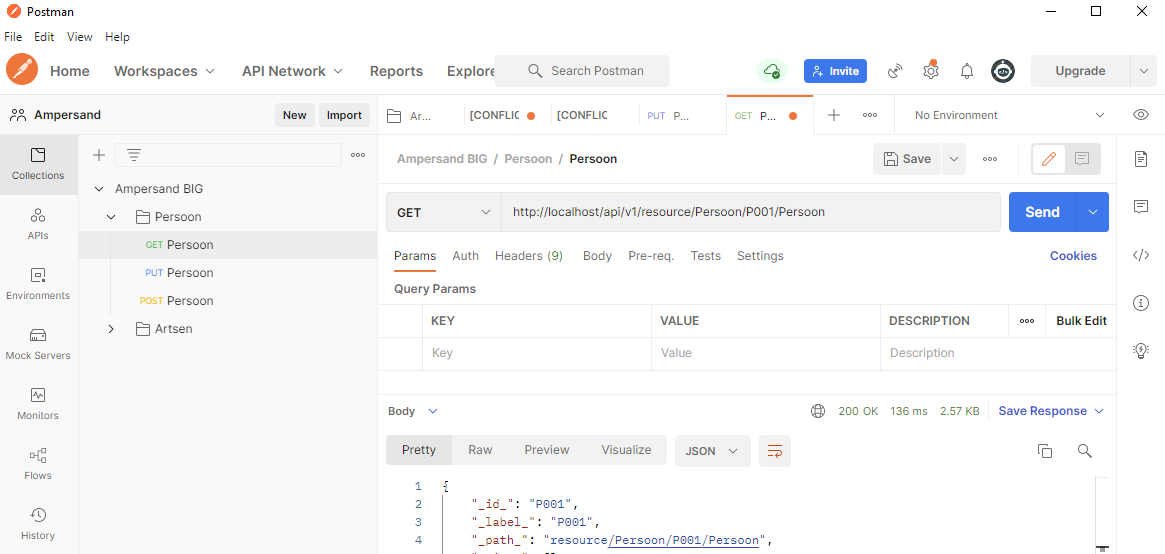
\includegraphics[width=\textwidth]{/postman_GET.PNG}
    \caption{Postman GET Person}
    \label{fig:postman-get-person}
\end{figure}

\paragraph{\textbf{Customization \acrshort{rk}}}\label{swot:o_customization}:
An organized ICT organization such as the \acrshort{cibg} has an architecture that new software must comply with.
One of the developments in the \acrshort{cibg} is the set-up of the \acrshort{rk} (see interview developer Appendix~\ref{par:interview-developer}).
\acrlong{rk} its terminology includes "zaken" and "producten".
Every service, read implementation of a law, we call a product.
There are default items that always appear in every registry.
These are pre-modeled in \acrshort{rk}.
This includes a foundation for each registry and can be expanded to meet the needs of the registry.
The basis is the minimum common denominator of the registers, extendable to specific elements arising from the law.
There is certainly overlap in the data obtained from the analysis of the great law and the \acrshort{rk}.
About 80\% of the \acrshort{rk} is generic and the other 20\% is custom.
All new registers therefore have the same basic principles and largely run on the same software.
However, a mapping still has to take place from the found Concepts from the law to \acrshort{rk}.
The overlap in this is not always immediately visible.
Within the \acrshort{rk} the term product is used, within the \acrshort{big} this product is a register or possibly even all registers.
The latter depends on the implementation.
This mapping must be made explicit and has not been taken into account in this study.
The developer has indicated that full integration of the Ampersand model is not possible, due to the aforementioned overlap of the Concepts.
However, the modified part of the \acrshort{rk} can be used for the Ampersand model implementation.
Although Ampersand is new to the \acrshort{cibg} organization, one of the interviewees pointed out (see interview analist~\ref{par:interview-analist}) that documentation in the form of a design should be made with each new register.
According to the analyst, it should not matter which tool is used for this.
The advantage of Ampersand is that it generates a model from the analysis instead of the usual model-to-text approach.
A model is made of each pattern.
See for example the Pattern for \mbox{Person} (see script~\ref{lst:persoon}).
This results in the model of figure~\ref{fig:pattern-persoon}.
\begin{figure}[H]
    \centering
        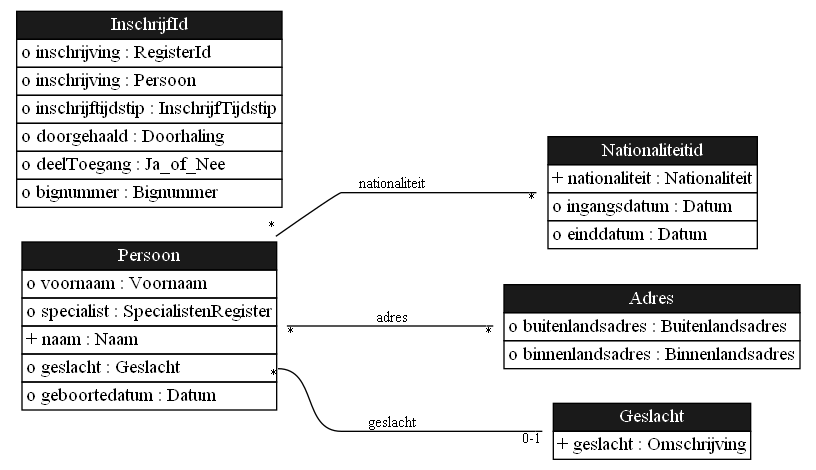
\includegraphics[width=1\textwidth]
            {../images/CDPatternPersoon.png}
        \caption{Pattern Persoon}
    \label{fig:pattern-persoon}
\end{figure}
Calculations are not standard in Ampersand, but this can be solved by writing external functions or even solving it in \acrshort{rk}.
(Ref. to  \nameref{s:5_2_demarcation}, \nameref{s:1_7_architecture_and_registerkern}, \nameref{s:4_1_architectural_fit}, \nameref{s:1_10_ampersand_design_method}, \nameref{s:2_7_organisation_ampersand_use}, \nameref{s:4_7_total_design})

\paragraph{\textbf{Version-gap analysis}}\label{swot:o_version_gap_analysis}:
Although it is not the intention to use Ampersand prototype in a production environment, it is useful to save the data entered in an earlier version and use it in later versions.
In ``\nameref{swot:w_data_migration}'' included with the weaknesses we indicate that this is a problem and it would be a good addition to develop a tool in Ampersand that focuses on preserving data across versions.
(Ref. to \nameref{s:3_5_model_maintenance})

\paragraph{\textbf{Atlas local}}\label{swot:o_atlas_local}:
In RAP there is a tool called Atlas, it shows the context and the patterns.
In addition, all Concepts, Rules, Properties and Relations, with hyperlinks to the components.
Via the hyperlink details of the item inclusion a relationship diagram is shown, very nicely executed and very useful when working in RAP.
This tool is a viewer on the information and it is not possible to also edit the \F{information in Atlas}{Being able to edit the Atlas information from Atlas}.
However, the case study was so large that the RAP environment was not sufficient.
RAP does not support Includes and has been used extensively.
Unfortunately, \F{Atlas availability}{Make Atlas available outside the RAP environment.} cannot be implemented outside of RAP.

As a novice user of Ampersand it takes a while to master Relation algebra.
That is why an excel sheet has been made to make the Relations visible with the associated multiplicity.
This is a method that is easy to use initially.
The disadvantage of this approach is the consistent transfer of Concepts and Relations.
We need to double track this information and redundancy in the field of data will certainly go wrong.
When Concepts disappear, they must also be removed from Excel or Relations that do change due to new insights must be adjusted here.
In short, this does work for small, well-arranged projects, but for larger ones, gaps will quickly arise and this no longer represents reality.
The result was that the excel sheet was used a lot in the beginning and not anymore later on.
(Ref. to \nameref{s:3_5_model_maintenance}, \nameref{s:2_2_multiplicity})

\paragraph{\textbf{\acrlong{ca} as testbasis}}\label{swot:o_ca_as_testbasis}:
By using Ampersand as a design tool, a prototype is available at an early stage.
This prototype can be converted into a website with the appearance of a \acrshort{cibg} website by means of HTML additions and CSS adjustments.
Test cases can already be developed at an early stage on the basis of this prototype and the functions of the prototype, by using the APIs, can be used as a stub in the development of the system.
(Ref. to \nameref{s:2_6_prototype_use}, \nameref{s:1_10_ampersand_design_method})

\paragraph{\textbf{Stub}}\label{swot:o_stub}:
The prototype can be accessed through APIs.
In principle it is possible to use the prototype in whole or in part as a stub.
When developing the application, based on the \acrshort{ca}, the prototype can be used in the form of a stub.
(Ref. to \nameref{s:4_5_test_scenario})


\paragraph{\textbf{Annotation}}\label{swot:o_annotation}:
To maintain an overview when performing the textual analysis, it is necessary to use a annotation (see section~\ref{subsection:ampersand-knowledge}, heading~\nameref{subsub:1_annotation}).
Annotation would be a nice addition to Ampersand.
It does introduce a close link between Ampersand and the source document.
(Ref. to \nameref{s:1_3_source_handling})

\subsubsection{Threats}\label{subsub:4_treaths}

\paragraph{\textbf{NIH}}\label{swot:t_nih}:
Ampersand is a completely new method for the \acrshort{cibg} organization.
People have never heard of it and unfortunately there is not much to be found about it.
That means that people are not positive about it in advance, and NIH calls it~\footnote{not invented here}\citep{antons_assessing_2017}.
The expectation of the organization is that the Ampersand method will take more time than the current method (see interview~\ref{int:I-1.8}) and people will be wary of something new.
Obviously, the advantages of the method are not yet understood.
Benefits such as working directly at the source, generating a prototype from there (see appendix~\ref{appendixPrototype}) with all validations and full conceptual specifications (see appendix~\ref{ConceptualAnalysis}).
Having a prototype makes it possible to build test scenarios at an early stage and with the \acrlong{ca} you can start building right away.
(Ref. to \nameref{s:4_5_test_scenario}, \nameref{s:2_6_prototype_use}, \nameref{s:1_11_law_effective})

\paragraph{\textbf{Process orientation}}\label{swot:t_process_orientation}:
Many organizations are process oriented.
With \acrshort{cibg}, the work instructions that the employees use are usually process steps that must be performed.
Also the design of systems such as \acrshort{zorro} are designed to support a process-oriented approach.
Ampersand supports a reactive focused approach.
This cannot be translated into process-oriented work instructions.
The challenge for the adoption of Ampersand therefore lies partly in the organization its ability to adapt from process-based to reactive.
Also contributing to this is that the adjacent system, \acrshort{rk}, is a process-oriented system, which supports a number of standard processes that affect (almost) every register.
(Ref. to \nameref{s:1_7_architecture_and_registerkern}, \nameref{s:5_1_registerkern}, \nameref{s:5_2_demarcation})

\paragraph{\textbf{Redundancy}}\label{swot:t_redundancy_script_tool}:
The reuse of Concepts, Relations and Rules is on the one hand a powerful means whereby consistency is enforced.
However, when using Ampersand, it is not always visible that components are already being used.
For example, it is possible to include these components several times in the analysis and to assign them a different definition each time.
While this should be detectable by Ampersand.
Conversely, it is also possible to rename components with the same definition.
Of course, Ampersand cannot control this.
The IDE used should support this, but it does not at the moment.
(Ref. to \nameref{s:5_2_demarcation})

\paragraph{\textbf{IDE-refactoring}}\label{swot:t_ide_refactoring}:
Ampersand as a tool is supported by an IDE.
For \acrshort{vsc} there is a plugin that supports the use of Ampersand.
In addition, the Ampersand tool is built in such a way that the compilation of the script from the \acrshort{vsc} is supported.
An omission in the use of \acrshort{vsc} is a refactoring option.
To be able to refactor, the IDE tool needs to know which components are used and where they are used.
This condition is not met, where refactoring is not possible in advance.
Not being able to refactor is a cause of causing redundancy in the code (see paragraph~\nameref{swot:t_redundancy_script_tool}).
(Ref. to \nameref{s:3_2_common_objects})





\newpage
\parindent0em
\begin{figure}[ht]
    \centering

    \begin{tikzpicture}[
        pentagon/.style={%
            shape=regular polygon, regular polygon sides=5, minimum size=7.3cm, inner
            sep=-1mm, draw, fill=lightgray!75!yellow
        }, font=\scriptsize\sffamily, thick
    ]
    
    % \draw[help lines] (-16,-16) grid (16,16);
    \filldraw[thin,gray,fill=gray!25] (-8,-8) rectangle (8,8);
    \filldraw[thin,gray,fill=white] (-7.15,-7.15) rectangle (7.15,7.15);
    \draw[thin,gray] (7.15,7.15)--(8,8) (-7.15,7.15)--(-8,8) (-7.15,-7.15)--(-8,-8)
    (7.15,-7.15)--(8,-8);
    
    % Strengths
    \draw[thin,gray] (-0.025,0.025)--(-7.05,0.025)--(-0.025,7.05)--cycle;
    \node[pentagon,rotate=0] at (-3.75,3.75) {
        \begin{varwidth}{\linewidth}
            \begin{itemize}[leftmargin=*,noitemsep]
                \item \nameref{swot:s_api_availability}
                \item \nameref{swot:s_prototype}
                \item \nameref{swot:s_no_technical_debt}
                \item \nameref{swot:s_low_code}
                \item \nameref{swot:s_reactive_approach}
                \item \nameref{swot:s_error_free_specifications}
                \item \nameref{swot:s_conceptual_analysis}
                \item \nameref{swot:s_team_effort}
            \end{itemize}
        \end{varwidth}
    };
    \draw (-4,2) node[rotate=0] {\large\textbf{Strengths}};
    
    % Weaknesses
    \draw[thin,gray] (0.025,0.025)--(7.05,0.025)--(0.025,7.05)--cycle;
    \node[pentagon,rotate=0] at (3.75,3.75) {
        \begin{varwidth}{\linewidth}
            \begin{itemize}[leftmargin=*,noitemsep]
                \item \nameref{swot:w_api_its_description}
                \item \nameref{swot:w_manual_mapping}
                \item \nameref{swot:w_data_migration}
                \item \nameref{swot:w_documentation}
            \end{itemize}
        \end{varwidth}
    };
    \draw (4,2) node[rotate=0] {\large\textbf{Weaknesses}};
    
    % Opportunities
    \draw[thin,gray] (-0.025,-0.025)--(-7.05,-0.025)--(-0.025,-7.05)--cycle;
    \node[pentagon,rotate=0] at (-3.75,-3.75) {
        \begin{varwidth}{\linewidth}
            \begin{itemize}[leftmargin=*,noitemsep]
                \item \nameref{swot:o_api_http_responsecode}
                \item \nameref{swot:o_customization}
                \item \nameref{swot:o_version_gap_analysis}
                \item \nameref{swot:o_atlas_local}
                \item \nameref{swot:o_ca_as_testbasis}
                \item \nameref{swot:o_stub}
                \item \nameref{swot:o_annotation}
            \end{itemize}
        \end{varwidth}
    };
    \draw (-4,-2) node[rotate=0] {\large\textbf{Opportunities}};
    
    % Threats
    \draw[thin,gray] (0.025,-0.025)--(7.05,-0.025)--(0.025,-7.05)--cycle;
    \node[pentagon,rotate=0] at (3.75,-3.75) {
        \begin{varwidth}{\linewidth}
            \begin{itemize}[leftmargin=*,noitemsep]
                \item \nameref{swot:t_nih}
                \item \nameref{swot:t_process_orientation}
                \item \nameref{swot:t_redundancy_script_tool}
                \item \nameref{swot:t_ide_refactoring}
            \end{itemize}
        \end{varwidth}
    };
    \draw (4,-2) node[rotate=0] {\large\textbf{Threats}};
    \draw(0,-7.55) node {\Large EXTERNAL};
    \draw(0,7.55) node {\Large INTERNAL};
    \draw(-7.55,0) node[rotate=90] {\Large POSITIVE};
    \draw(7.55,0) node[rotate=270] {\Large NEGATIVE};
    \draw(-0.6,0.6) node {\Huge\textbf{S}}; 
    \draw(0.6,0.6) node {\Huge\textbf{W}};
    \draw(-0.6,-0.6) node {\Huge\textbf{O}};
    \draw(0.6,-0.6) node {\Huge\textbf{T}};
    \end{tikzpicture}
    \caption{SWOT Ampersand for government organization}
    \label{fig:swot}
\end{figure}

\parindent2em

The design of register systems has no specific points for attention.
Part of the research question was about designing for register systems.
Other than the source specific link, the \acrshort{big}, no particulars were found for registry systems.
The translation of this law into an information system results in a register.
The requirements of the register are laid down by law.
This concerned, among other things, the identifying data of a registration and in Article 3, paragraph 1~\footnote{\url{https://wetten.overheid.nl/jci1.3:c:BWBR0006251&hoofdstuk=II&paragraaf=1&article=3&z=2022-04-01&g=2022-04-01}} it says it is about multiple registers.
This also explains why there are few observations about registration systems.
The register system therefore does not stand alone, but is a consequence of the fact that the source is a law.